
\documentclass{beamer}
\mode<presentation>{
\usefonttheme{professionalfonts}
\useinnertheme{rounded}
\useoutertheme[subsection=false,footline=authortitle]{miniframes}
%Inner Color Themes
\usecolortheme{dolphin}
%	\usecolortheme{seahorse}


%Outer Color Themes
	\usecolortheme{rose}
%\usecolortheme{orchid}
}

%Typical documenttypes: article/book
%some examples:
%\documentclass[reqno,11pt]{book}   %%%for books
%\documentclass[]{minimal}			%%%for Minimal Working Example






%%%%%%%%%%%%%%%%%%%% setting for fast compiling

%\special{dvipdfmx:config z 0}		% no compression

\includeonly{chapters/chapter9}		% In practice, use an empty document called "chapter9"	% usually for printing books






%%%%%%%%%%%%%%%%%%%% here we include packages

%%%basic packages for math articles
\usepackage{amssymb}
\usepackage{amsthm}
\usepackage{amsmath}
\usepackage{amsfonts}
%\usepackage[shortlabels]{enumitem}	% It supersedes both enumerate and mdwlist. The package option shortlabels is included to configure the labels like in enumerate.

%%%packages for special symbols
\usepackage{pifont}					% Access to PostScript standard Symbol and Dingbats fonts
\usepackage{wasysym}				% additional characters
\usepackage{bm}						% bold fonts: \bm{...}
\usepackage{extarrows}				% may be replaced by tikz-cd
%\usepackage{unicode-math}			% unicode maths for math fonts, now I don't know how to include it

%%%basic packages for fancy electronic documents
%\usepackage[colorlinks]{hyperref}
%\usepackage[table,hyperref]{xcolor} 			% before tikz-cd. 
%\usepackage[table,hyperref,monochrome]{xcolor}	% disable colored output (black and white)

%%%packages for figures and tables (general setting)
\usepackage{float}				%Improved interface for floating objects
\usepackage{caption,subcaption}
\usepackage{adjustbox}			% for me it is usually used in tables 
\usepackage{stackengine}		%baseline changes

%%%packages for commutative diagrams
\usepackage{tikz-cd}
%\usepackage{quiver}			% see https://q.uiver.app/

%%%packages for pictures
\usepackage[width=0.5,tiewidth=0.7]{strands}
\usepackage{graphicx}			% Enhanced support for graphics

%%%packages for tables and general settings
\usepackage{array}
\usepackage{makecell}
\usepackage{multicol}
\usepackage{multirow}
\usepackage{diagbox}









%https://tex.stackexchange.com/questions/58852/possible-incompatibility-with-enumitem










%%%%%%%%%%%%%%%%%%%% here we include theoremstyles

\numberwithin{equation}{section}

\theoremstyle{plain}
%\newtheorem{theorem}{Theorem}[section]

\newtheorem{setting}[theorem]{Setting}
%\newtheorem{definition}[theorem]{Definition}
%\newtheorem{lemma}[theorem]{Lemma}
\newtheorem{proposition}[theorem]{Proposition}
%\newtheorem{corollary}[theorem]{Corollary}
\newtheorem{conjecture}[theorem]{Conjecture}

\newtheorem{claim}[theorem]{Claim}
\newtheorem{eg}[theorem]{Example}
\newtheorem{ex}[theorem]{Exercise}
%\newtheorem{fact}[theorem]{Fact}
\newtheorem{ques}[theorem]{Question}
\newtheorem{warning}[theorem]{Warning}



\newtheorem*{bbox}{Black box}
\newtheorem*{notation}{Conventions and Notations}


\numberwithin{equation}{section}


\theoremstyle{remark}

\newtheorem{remark}[theorem]{Remark}
\newtheorem*{remarks}{Remarks}

%%% for important theorems
%\newtheoremstyle{theoremletter}{4mm}{1mm}{\itshape}{ }{\bfseries}{}{ }{}
%\theoremstyle{theoremletter}
%\newtheorem{theoremA}{Theorem}
%\renewcommand{\thetheoremA}{A}
%\newtheorem{theoremB}{Theorem}
%\renewcommand{\thetheoremB}{B}

\newtheorem{short}{ }





%%%%%%%%%%%%%%%%%%%% here we declare some symbols

%%%%%%%DeclareMathOperator
%see here for why newcommand is better for DeclareMathOperator: https://tex.stackexchange.com/questions/67506/newcommand-vs-declaremathoperator

%%%%%basic symbols. Keep them!

%%%symbols for sets and maps
\DeclareMathOperator{\pt}{\operatorname{pt}}	%points. Other possibilities are \{pt\}, ...
\DeclareMathOperator{\Id}{\operatorname{Id}}	%identity in groups.
\DeclareMathOperator{\Img}{\operatorname{Im}}

\DeclareMathOperator{\Ob}{\operatorname{Ob}}
\DeclareMathOperator{\Mor}{\operatorname{Mor}}	%difference of Mor and Hom: Hom is usually for abelian categories
\DeclareMathOperator{\Hom}{\operatorname{Hom}}	\DeclareMathOperator{\End}{\operatorname{End}}
\DeclareMathOperator{\Aut}{\operatorname{Aut}}

%%%symbols for linear algebras and 
%%linear algebras
\DeclareMathOperator{\tr}{\operatorname{tr}}
\DeclareMathOperator{\diag}{\operatorname{diag}}	%for diagonal matrices

%%abstract algebras
\DeclareMathOperator{\ord}{\operatorname{ord}}
\DeclareMathOperator{\gr}{\operatorname{gr}}
\DeclareMathOperator{\Frac}{\operatorname{Frac}}

%%%symbols for basic geometries
\DeclareMathOperator{\vol}{\operatorname{vol}}	%volume
\DeclareMathOperator{\dist}{\operatorname{dist}}
\DeclareMathOperator{\supp}{\operatorname{supp}}

%%%symbols for category
%%names of categories
\DeclareMathOperator{\Mod}{\operatorname{Mod}}
\DeclareMathOperator{\Vect}{\operatorname{Vect}}
\DeclareMathOperator{\rep}{\operatorname{rep}} %usually rep means the category of finite dimensional representations, while Rep means the category of representations.
\DeclareMathOperator{\Rep}{\operatorname{Rep}}


%%%symbols for homological algebras
\DeclareMathOperator{\Tor}{\operatorname{Tor}}
\DeclareMathOperator{\Ext}{\operatorname{Ext}}
\DeclareMathOperator{\gldim}{\operatorname{gl.dim}}
\DeclareMathOperator{\projdim}{\operatorname{proj.dim}}
\DeclareMathOperator{\injdim}{\operatorname{inj.dim}}
\DeclareMathOperator{\rad}{\operatorname{rad}}


%%%symbols for algebraic groups
\DeclareMathOperator{\GL}{\operatorname{GL}}
\DeclareMathOperator{\SL}{\operatorname{SL}}

%%%symbols for typical varieties
\DeclareMathOperator{\Gr}{\operatorname{Gr}}
\DeclareMathOperator{\Flag}{\operatorname{Flag}}

%%%symbols for basic algebraic geometry
\DeclareMathOperator{\Spec}{\operatorname{Spec}}
\DeclareMathOperator{\Coh}{\operatorname{Coh}}
\newcommand{\Dcoh}{\mathcal{D}_{\operatorname{Coh}}}%%%This one shows the difference between \DeclareMathOperator and \newcommand
\DeclareMathOperator{\Pic}{\operatorname{Pic}}
\DeclareMathOperator{\Jac}{\operatorname{Jac}}

%%%%%advanced symbols. Choose the part you need!

%%%symbols for algebraic representation theory
\DeclareMathOperator{\Irr}{\operatorname{Irr}}
\DeclareMathOperator{\ind}{\operatorname{ind}}	%\ind(Q) means the set of  equivalence classes of finite dimensional indecomposable representations
\DeclareMathOperator{\Res}{\operatorname{Res}}
\DeclareMathOperator{\Ind}{\operatorname{Ind}}
\DeclareMathOperator{\cInd}{\operatorname{c-Ind}}


%%%symbols for algebraic topology
\DeclareMathOperator{\EGG}{\operatorname{E}\!}
\DeclareMathOperator{\BGG}{\operatorname{B}\!}

\DeclareMathOperator{\chern}{\operatorname{ch}^{*}}
\DeclareMathOperator{\Td}{\operatorname{Td}}
\DeclareMathOperator{\AS}{\operatorname{AS}}	%Atiyah--Segal completion theorem 

%%%symbols for Auslander--Reiten theory 
\DeclareMathOperator{\Modup}{\overline{\operatorname{mod}}}
\DeclareMathOperator{\Moddown}{\underline{\operatorname{mod}}}
\DeclareMathOperator{\Homup}{\overline{\operatorname{Hom}}}
\DeclareMathOperator{\Homdown}{\underline{\operatorname{Hom}}}


%%%symbols for operad
\DeclareMathOperator{\Com}{\operatorname{\mathcal{C}om}}
\DeclareMathOperator{\Ass}{\operatorname{\mathcal{A}ss}}
\DeclareMathOperator{\Lie}{\operatorname{\mathcal{L}ie}}
\DeclareMathOperator{\calEnd}{\operatorname{\mathcal{E}nd}} %cal=\mathcal


%%%%%personal symbols. Use at your own risk!

%%%symbols only for master thesis
\DeclareMathOperator{\ptt}{\operatorname{par}}	%the partition map
\DeclareMathOperator{\str}{\operatorname{str}}	%strict case
\DeclareMathOperator{\RRep}{\widetilde{\operatorname{Rep}}}
\DeclareMathOperator{\Rpt}{\operatorname{R}}
\DeclareMathOperator{\Rptc}{\operatorname{\mathcal{R}}}
\DeclareMathOperator{\Spt}{\operatorname{S}}
\DeclareMathOperator{\Sptc}{\operatorname{\mathcal{S}}}
\DeclareMathOperator{\Kcurl}{\operatorname{\mathcal{K}}}
\DeclareMathOperator{\Hcurl}{\operatorname{\mathcal{H}}}
\DeclareMathOperator{\eu}{\operatorname{eu}}
\DeclareMathOperator{\Eu}{\operatorname{Eu}}
\DeclareMathOperator{\dimv}{\operatorname{\underline{\mathbf{dim}}}}
\DeclareMathOperator{\St}{\mathcal{Z}}

%%%%%symbols which haven't been classified. Add your own math operators here!


\DeclareMathOperator{\Modr}{\operatorname{-Mod}}
\DeclareMathOperator{\BM}{\operatorname{BM}}




%%%%%%%newcommand

%%%basic symbols
\newcommand{\norm}[1]{\Vert{#1}\Vert}

%%%symbols only for master thesis
\newcommand{\dimvec}[1]{\mathbf{#1}}
\newcommand{\abdimvec}[1]{|\dimvec{#1}|}
\newcommand{\ftdimvec}[1]{\underline{\dimvec{#1}}}

\newcommand{\absgp}[1]{\mathbb{#1}}
\newcommand{\WWd}{\absgp{W}_{\abdimvec{d}}}
\newcommand{\Wd}{W_{\dimvec{d}}}
\newcommand{\ww}{\varpi}
\newcommand{\MinWd}{\operatorname{Min}(\absgp{W}_{\abdimvec{d}},W_{\dimvec{d}})}
\newcommand{\Compd}{\operatorname{Comp}_{\dimvec{d}}}
\newcommand{\Shuffled}{\operatorname{Shuffle}_{\dimvec{d}}}


\newcommand{\Omcell}{\Omega}
\newcommand{\OOmcell}{\boldsymbol{\Omega}}
\newcommand{\Vcell}{\mathcal{V}}
\newcommand{\VVcell}{\boldsymbol{\mathcal{V}}}
\newcommand{\Ocell}{\mathcal{O}}
\newcommand{\OOcell}{\boldsymbol{\mathcal{O}}}
\newcommand{\preimage}[1]{\widetilde{#1}}
\newcommand{\orde}{\operatorname{ord}_e}
\newcommand{\fakestar}{*}

%as the subscription of Hom
\newcommand{\Alggp}{\text{-Alg gp}}







%%%%%%%%%%%%%%%%%%%% here we make some blocks for special features. 

%%%% todo notes %%%%
\usepackage[colorinlistoftodos,textsize=footnotesize]{todonotes}
\setlength{\marginparwidth}{2.5cm}
\newcommand{\leftnote}[1]{\reversemarginpar\marginnote{\footnotesize #1}}
\newcommand{\rightnote}[1]{\normalmarginpar\marginnote{\footnotesize #1}\reversemarginpar}









%%%%%%%%%%%%%%%%%%%% here we make some global settings. Understand everything here before you make a document!

%\usepackage[a4paper,left=3cm,right=3cm,bottom=4cm]{geometry}
%\usepackage{indentfirst}	% Indent first paragraph after section header

\setcounter{tocdepth}{2}


%https://latexref.xyz/_005cparindent-_0026-_005cparskip.html
\setlength{\parindent}{15pt}	
\setlength{\parskip}{0pt plus1pt}

%\setlength\intextsep{0cm}
%\setlength\textfloatsep{0cm}
\def\arraystretch{1}
%\setcounter{secnumdepth}{3}

\allowdisplaybreaks



% 设置图形文件的搜索路径


\graphicspath{{../figures/}}

\usepackage[T1]{fontenc}
\begin{document}

% The beginning depends on the documentclass. Rewrite this part if you use different documentclass!


\title{Affine pavings of partial flag varieties}
\author[Xiaoxiang Zhou]{Xiaoxiang Zhou\\[10mm]{\small Advisor: Prof. Dr. Catharina Stroppel \\ Second Advisor: Dr. Jens Niklas Eberhardt}}
\institute[Bonn uni]{Universität Bonn}
\date{\today}

\begin{frame}
\titlepage
\end{frame}
\begin{frame}{Process}
\tableofcontents[hideallsubsections]
\end{frame}
\section{Setting and Statement}
\begin{frame}{Process}
\tableofcontents[currentsection,hideallsubsections]
\end{frame}
\begin{frame}[fragile]{Affine paving}
\begin{setting}
$K= \mathbb{C}$, $X$: algebraic variety over $K$. 
\end{setting}
\begin{definition}
An \textbf{affine paving} of $X$ is a filtration
$$0= X_0 \subset X_1 \subset \cdots \subset X_d=X$$
with $X_i$ closed and $X_{i+1} \setminus X_i \cong \mathbb{A}^k_{K}$.
\end{definition}
\begin{figure}[th]
	\begin{minipage}[b]{.45\textwidth}
		\centering
		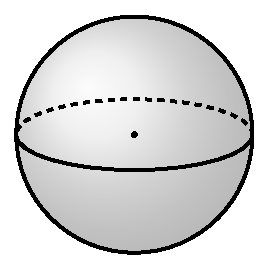
\includegraphics[width=.3\textwidth]{figures/sphere/Sphere1.pdf}
		$$\mathbb{P}^1= \{ \infty \} \sqcup \mathbb{A}^1$$
	\end{minipage}
	\begin{minipage}[b]{.45\textwidth}
	\centering
	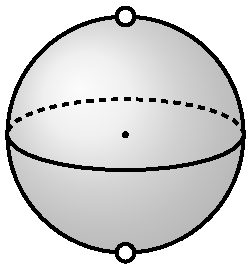
\includegraphics[width=.3\textwidth]{figures/sphere/Sphere3.pdf}
	$$\mathbb{P}^1 \smallsetminus \{0,\infty \} \text{ has no affine paving}$$
\end{minipage}
\end{figure}

\end{frame}

\begin{frame}[fragile]{Quiver and quiver representation}

Quiver is a graph. It has some vertices $\&$ arrows.\\

In this talk, all the quivers are finite and connected.

\end{frame}

\begin{frame}[fragile]{Quiver and quiver representation}

We focus on the Dynkin quiver.\\

That means, the graph of the Dynkin diagrams in the ADE series.

\end{frame}

%https://tex.stackexchange.com/questions/436284/how-to-adjust-parenthesis-thickness-without-changing-the-font
%https://tex.stackexchange.com/questions/207056/wrong-too-much-vertical-space-above-vdots-in-small-matrix
\begin{frame}[fragile]{Partial flag variety}
\begin{definition}
Fix a quiver $Q$ and $M \in \rep(Q)$,
\begin{equation*}
\begin{aligned}
  \Flag_{d}(M)\colon=\;& \left\{ F\colon 0 \subseteq N_1 \subseteq \cdots\subseteq N_d \subseteq M  \right\} \\ 
  \Flag_{\ftdimvec{f}}(M)\colon=\;&\left\{ F\colon 0 \subseteq N_1 \subseteq \cdots\subseteq N_d \subseteq M \;\middle|\;\rule{0mm}{3.4mm} \dimv M_i =\ftdimvec{f}_i \right\}
\end{aligned}
\end{equation*}
\end{definition}
\begin{eg}
$Q= \bullet$, $M=\mathbb{C}^n$, $\ftdimvec{f}:=\left(
    \begin{smallmatrix}
    n \\ \vphantom{\int\limits^x}\smash{\vdots} \\ 1
    \end{smallmatrix}
    \right)$
\begin{equation*}
\begin{aligned}
  \Flag_{d}(\mathbb{C}^n)=\;& \left\{ F\colon 0 \subseteq N_1 \subseteq \cdots\subseteq N_d \subseteq \mathbb{C}^n  \right\}\hspace{-10mm}& \\ 
    \Flag_{1}(\mathbb{C}^n)=\;& \left\{ F\colon 0 \subseteq N_1  \subseteq \mathbb{C}^n  \right\} &= \sqcup_{k=0}^{n} \Gr (n,k) \\
    \Flag_{\ftdimvec{f}}(\mathbb{C}^n)=\;&\text{ complete flags of $\mathbb{C}^n$} & \\
    \Flag_{(\!k\!)\!}(\mathbb{C}^n)=\;& \Gr (n,k) &\\
\end{aligned}
\end{equation*}
\end{eg}

\end{frame}


\begin{frame}[fragile]{Statement}
\begin{theorem}
For a Dynkin quiver $Q$ and $M \in \rep(Q)$, 
$$\Flag_{d}(M) \text{ has an affine paving.}$$
\end{theorem}

\end{frame}


%%%%%%%%%%%%%%%%%%%%%%%%%%%%%%%%%%%%
\section{Case study}
\begin{frame}{Process}
\tableofcontents[currentsection,hideallsubsections]
\end{frame}


\begin{frame}[fragile]{Task 1. $Q= \bullet$, $M=\mathbb{C}^n$}

In this case,
% https://q.uiver.app/?q=WzAsOSxbMCwwLCJcXEdMX24oXFxtYXRoYmJ7Q30pIFxcLFxccm90YXRlYm94W29yaWdpbj1jXXsyNzB9eyRcXGNpcmNsZWFycm93cmlnaHQkfVxcOyBcXG1hdGhiYntDfV5uIl0sWzMsMCwiXFxHTF9uKFxcbWF0aGJie0N9KSAiXSxbMywxLCJCICJdLFsyLDFdLFs0LDEsIlxccm90YXRlYm94W29yaWdpbj1jXXsyNzB9eyRcXGNpcmNsZWFycm93cmlnaHQkfVxcOyBcXEZsYWdfe2R9KFxcbWF0aGJie0N9Xm4pIl0sWzQsMCwiXFxyb3RhdGVib3hbb3JpZ2luPWNdezI3MH17JFxcY2lyY2xlYXJyb3dyaWdodCR9XFw7IFxcRmxhZ197ZH0oXFxtYXRoYmJ7Q31ebikiXSxbMSwwXSxbMiwwXSxbMSwxXSxbNiw3LCIiLDAseyJzdHlsZSI6eyJib2R5Ijp7Im5hbWUiOiJzcXVpZ2dseSJ9fX1dLFs4LDMsIiIsMCx7InN0eWxlIjp7ImJvZHkiOnsibmFtZSI6InNxdWlnZ2x5In19fV1d
\[\begin{tikzcd}[row sep=0mm, column sep=0mm]
	{\GL_n(\mathbb{C}) \,\rotatebox[origin=c]{270}{$\circlearrowright$}\; \mathbb{C}^n} & {} &[20mm] {} & {\GL_n(\mathbb{C}) } &[-3mm] {\rotatebox[origin=c]{270}{$\circlearrowright$}\; \Flag_{d}(\mathbb{C}^n)} \\
	& {} & {} & {B } & {\rotatebox[origin=c]{270}{$\circlearrowright$}\; \Flag_{d}(\mathbb{C}^n)}
	\arrow[squiggly, from=1-2, to=1-3]
	\arrow[squiggly, from=2-2, to=2-3]
\end{tikzcd}\]

$\Flag_{d}(\mathbb{C}^n)$ has an affine paving given by Schubert cells (i.e., $B$-orbits).

\begin{block}{Note}
When $Q= \bullet \longrightarrow \bullet$, $\Flag_{\dimvec{f}}(M)$ have no natural group actions.
\end{block}


\end{frame}


\begin{frame}[fragile]{Idea of affine pavings}
Find a nice short exact sequence 
$$0\longrightarrow X \stackrel{\iota}{\longrightarrow} M \stackrel{\pi}{\longrightarrow} S \longrightarrow 0$$
which induces a nice morphism
\begin{equation*}
\begin{aligned}
\Psi: \Flag_{d}(M) \longrightarrow\;& \Flag_{d}(X) \times \Flag_{d}(S) \\ 
F\hspace{5mm} \longmapsto\;& \hspace{5mm}\left( \iota^{-1}(F), \pi(F) \right)
\end{aligned}
\end{equation*}
We construct the affine paving of $\Flag_{d}(M)$ from the affine paving of $\Flag_{d}(X)$ and $\Flag_{d}(S)$. Then, we use mathematical induction.
\end{frame}



%%%%%%%%%%%%%%%%%%%%%%%%%%%%%%%%%%%%%%%%%%%%%
\section{Auslander--Reiten theory}
\begin{frame}{Process}
\tableofcontents[currentsection,hideallsubsections]
\end{frame}
\begin{frame}[fragile]{Another example: $D_4 \qquad$% https://q.uiver.app/?q=WzAsNCxbMCwxLCIxIl0sWzEsMSwiMiJdLFsyLDEsIjMiXSxbMSwwLCI0Il0sWzAsMV0sWzIsMV0sWzMsMV1d
\begin{tikzcd}[sep={3mm},font = \small, ampersand replacement=\&]
\& 4 \\
1 \& 2 \& 3
\arrow[from=2-1, to=2-2]
\arrow[from=2-3, to=2-2]
\arrow[from=1-2, to=2-2]
\end{tikzcd}}

\begin{overlayarea}{\linewidth}{\textheight}
\begin{short}
\adjustbox{minipage=[b][1.3\textheight][t]{2\paperwidth},scale=0.5,center}{%
% https://q.uiver.app/?q=WzAsNCxbMCwwLCIxIl0sWzEsMSwiMiJdLFsyLDAsIjMiXSxbMywwLCI0Il0sWzAsMV0sWzIsMV0sWzMsMV1d
\[\begin{tikzcd}[column sep={2cm,between origins},row sep={8mm,between origins}]
1 &&[-15mm] 3 & 4 \\
& 2
\arrow[from=1-1, to=2-2]
\arrow[from=1-3, to=2-2]
\arrow[from=1-4, to=2-2]
\end{tikzcd}\]

\vspace{5mm}
% https://q.uiver.app/?q=WzAsMTIsWzEsMCwiXFxzdWJzdGFja3swXFxcXDAxMH0iXSxbMCwxLCJcXHN1YnN0YWNrezBcXFxcMTEwfSJdLFsyLDEsIlxcc3Vic3RhY2t7MFxcXFwwMTF9Il0sWzMsMSwiXFxzdWJzdGFja3sxXFxcXDAxMH0iXSxbMSwyLCJcXHN1YnN0YWNrezFcXFxcMTIxfSJdLFswLDMsIlxcc3Vic3RhY2t7MVxcXFwwMTF9Il0sWzIsMywiXFxzdWJzdGFja3sxXFxcXDExMH0iXSxbMywzLCJcXHN1YnN0YWNrezBcXFxcMTExfSJdLFswLDUsIlxcc3Vic3RhY2t7MFxcXFwxMDB9Il0sWzIsNSwiXFxzdWJzdGFja3swXFxcXDAwMX0iXSxbMyw1LCJcXHN1YnN0YWNrezFcXFxcMDAwfSJdLFsxLDQsIlxcc3Vic3RhY2t7MVxcXFwxMTF9Il0sWzAsMV0sWzAsMl0sWzAsM10sWzEsNF0sWzIsNF0sWzMsNF0sWzQsNV0sWzQsNl0sWzQsN10sWzUsMTFdLFs2LDExXSxbNywxMV0sWzExLDhdLFsxMSw5XSxbMTEsMTBdXQ==
\[\begin{tikzcd}[column sep={2cm,between origins},row sep={13mm,between origins}]
& {\substack{0\\010}}&[-15mm]& \\
{\substack{0\\110}} && {\substack{0\\011}} & {\substack{1\\010}} \\
& {\substack{1\\121}} \\
{\substack{1\\011}} && {\substack{1\\110}} & {\substack{0\\111}} \\
& {\substack{1\\111}} \\
{\substack{0\\100}} && {\substack{0\\001}} & {\substack{1\\000}}
\arrow[from=1-2, to=2-1]
\arrow[from=1-2, to=2-3]
\arrow[from=1-2, to=2-4]
\arrow[from=2-1, to=3-2]
\arrow[from=2-3, to=3-2]
\arrow[from=2-4, to=3-2]
\arrow[from=3-2, to=4-1]
\arrow[from=3-2, to=4-3]
\arrow[from=3-2, to=4-4]
\arrow[from=4-1, to=5-2]
\arrow[from=4-3, to=5-2]
\arrow[from=4-4, to=5-2]
\arrow[from=5-2, to=6-1]
\arrow[from=5-2, to=6-3]
\arrow[from=5-2, to=6-4]
\end{tikzcd}\]
}
For other examples, see \href{https://github.com/ramified/personal_handwritten_collection/raw/c5f6429469b144c8ba72a0ca41f45d70ff8a2709/weeklyupdate/2021.08.15_indec_rep_of_Dynkinquiver.pdf}{here}.
\end{short}


\end{overlayarea}
\end{frame}


%%%%%%%%%%%%%%%%%%%%%%%%%%%%%%%%%%%%%%%%%%%%%%%
\section{Sketch of proof}
\begin{frame}{Process}
\tableofcontents[currentsection,hideallsubsections]
\end{frame}



\end{document}